\documentclass[]{article}
\usepackage{lmodern}
\usepackage{amssymb,amsmath}
\usepackage{ifxetex,ifluatex}
\usepackage{fixltx2e} % provides \textsubscript
\ifnum 0\ifxetex 1\fi\ifluatex 1\fi=0 % if pdftex
  \usepackage[T1]{fontenc}
  \usepackage[utf8]{inputenc}
\else % if luatex or xelatex
  \ifxetex
    \usepackage{mathspec}
  \else
    \usepackage{fontspec}
  \fi
  \defaultfontfeatures{Ligatures=TeX,Scale=MatchLowercase}
\fi
% use upquote if available, for straight quotes in verbatim environments
\IfFileExists{upquote.sty}{\usepackage{upquote}}{}
% use microtype if available
\IfFileExists{microtype.sty}{%
\usepackage{microtype}
\UseMicrotypeSet[protrusion]{basicmath} % disable protrusion for tt fonts
}{}
\usepackage[margin=1in]{geometry}
\usepackage{hyperref}
\hypersetup{unicode=true,
            pdfborder={0 0 0},
            breaklinks=true}
\urlstyle{same}  % don't use monospace font for urls
\usepackage{graphicx,grffile}
\makeatletter
\def\maxwidth{\ifdim\Gin@nat@width>\linewidth\linewidth\else\Gin@nat@width\fi}
\def\maxheight{\ifdim\Gin@nat@height>\textheight\textheight\else\Gin@nat@height\fi}
\makeatother
% Scale images if necessary, so that they will not overflow the page
% margins by default, and it is still possible to overwrite the defaults
% using explicit options in \includegraphics[width, height, ...]{}
\setkeys{Gin}{width=\maxwidth,height=\maxheight,keepaspectratio}
\IfFileExists{parskip.sty}{%
\usepackage{parskip}
}{% else
\setlength{\parindent}{0pt}
\setlength{\parskip}{6pt plus 2pt minus 1pt}
}
\setlength{\emergencystretch}{3em}  % prevent overfull lines
\providecommand{\tightlist}{%
  \setlength{\itemsep}{0pt}\setlength{\parskip}{0pt}}
\setcounter{secnumdepth}{0}
% Redefines (sub)paragraphs to behave more like sections
\ifx\paragraph\undefined\else
\let\oldparagraph\paragraph
\renewcommand{\paragraph}[1]{\oldparagraph{#1}\mbox{}}
\fi
\ifx\subparagraph\undefined\else
\let\oldsubparagraph\subparagraph
\renewcommand{\subparagraph}[1]{\oldsubparagraph{#1}\mbox{}}
\fi

%%% Use protect on footnotes to avoid problems with footnotes in titles
\let\rmarkdownfootnote\footnote%
\def\footnote{\protect\rmarkdownfootnote}

%%% Change title format to be more compact
\usepackage{titling}

% Create subtitle command for use in maketitle
\newcommand{\subtitle}[1]{
  \posttitle{
    \begin{center}\large#1\end{center}
    }
}

\setlength{\droptitle}{-2em}
  \title{}
  \pretitle{\vspace{\droptitle}}
  \posttitle{}
  \author{}
  \preauthor{}\postauthor{}
  \date{}
  \predate{}\postdate{}


\begin{document}

The following section will introduce the data and its sources. We use
the Chapel Hill Expert Survey (CHES) on European party position in order
to construct our dependent variable of \emph{Support for Populist
Parties} (i.e.~Support for Progressive or Traditionalist Populist
parties) along with individual level data from the European Social
Survey (ESS) (Section 3.1). The following subsection operationalizes our
hypotheses (cultural and economic explanations for populism) and
subsequently a description of the used control variables is given
(Section 3.2). Following this, the statistical methodology is explained
(Section 3.3) and a short examination of descriptive statistics takes
place (Section 3.4). Lastly, the results of estimated multinomial
logistic regression models are reported and examined for their
implications regarding the research hypotheses (Section 3.5).

\subsection{Data \& Operationalization}\label{data-operationalization}

The CHES dataset contains information on the positions of XXX political
parties in 40 European countries on european and national policy issues
in the timerange between 1999 and 2014. This makes the CHES data
suitable for identifying the ideological party positions that can be
classified as progressive and traditionalist populism within the
European context.

As a first step, we selected two variables that are in line with our
minimalistic definition of populism. They will be used to construct the
an Establishment - Anti-Establishment Axis.

\subsubsection{Establishment - Anti-Establishment
Axis}\label{establishment---anti-establishment-axis}

Populism, as it is conceptualized in this study, is characterized by two
main features: a disdain for the established elites that supposedly
exploit the \emph{pure} and \emph{little} people and an opposition to
the effects of globalization that brings cultures and economies closer
together at the expense of the (local) working class.

\textbf{Anti-Elite Sentiment}

Anti-Elite Sentiment is measured with the 11-point scale (0-1) variable
\emph{antielite\_salience} that indicates the salience of anti-elite
rhetoric within a given party. This corresponds with Mudde and
Kaltwasser's concept of populism where the ``corrupt elite'' is pitted
against the pure people (M/K 2017: 12).

\begin{itemize}
\tightlist
\item
  \emph{Salience of anti-establishment and anti-elite rhetoric}

  \begin{enumerate}
  \def\labelenumi{\arabic{enumi}.}
  \setcounter{enumi}{-1}
  \tightlist
  \item
    Not important at all
  \item
    Extremely important
  \end{enumerate}
\end{itemize}

\textbf{Euroskepticism}

Euroskepticism (\emph{position}\footnote{The Euroskepticism variable has
  been recoded so that higher values indicate higher opposition to
  European integration.}) will be used as a proxy variable for
anti-globalization. Populists are consistently opposed to the European
integration process, albeit for different reasons.

\begin{itemize}
\tightlist
\item
  \emph{Overall orientation of the party leadership towards European
  integration}

  \begin{enumerate}
  \def\labelenumi{\arabic{enumi}.}
  \tightlist
  \item
    Strongly opposed
  \item
    Strongly in favor
  \end{enumerate}
\end{itemize}

\subsubsection{Progressivism - Traditionalism
Axis}\label{progressivism---traditionalism-axis}

Next, we try to identify the value cleavage between progressivism and
traditionalism.

This value cleavage depicted divides \emph{progressives}, who favor
progressive social values, promote liberal lifestyles and acceptance of
homosexuality, civil liberties and multiculturalism from
\emph{traditionalists} who take the opposite stance on of all these
positions. The following Variables have been selected in order to
distinguish between progressive and traditionalist populism.

\textbf{GAL-TAN}

GAL-TAN is a new politics dimension invented by @hooghe2002does. The
capital letters are abbrevations for a scale that is supposed to capture
the new fault lines in European politics and they stand for
\emph{Green-Alternative-Libertarian} (GAL) and
\emph{Traditional-Authoritarian-Nationalist} (TAN) respectively.

\begin{itemize}
\tightlist
\item
  \emph{Position of the party {[}\ldots{}{]} in terms of their views on
  democratic freedoms and rights. ``Libertarian'' or ``postmaterialist''
  parties favor expanded personal freedoms, for example, access to
  abortion, active euthanasia, same-sex marriage, or greater democratic
  participation. ``Traditional'' or ``authoritarian'' parties often
  reject these ideas; they value order, tradition, and stability, and
  believe that the government should be a firm moral authority on social
  and cultural issues (galtan).}

  \begin{enumerate}
  \def\labelenumi{\arabic{enumi}.}
  \setcounter{enumi}{-1}
  \tightlist
  \item
    Libertarian/Postmaterialist
  \item
    Center
  \item
    Traditional/Authoritarian
  \end{enumerate}
\end{itemize}

\textbf{Social Lifestyle}

The acceptance of different lifestyle is a phenomena that consistently
splits traditionalists from progressives. While progressives push for
the acceptance of non-traditional social lifestyles traditionalists see
this push as undermining very fabric of society.

\begin{itemize}
\tightlist
\item
  \emph{Position on social lifestyle (e.g.~homosexuality)
  (sociallifestyle).}

  \begin{enumerate}
  \def\labelenumi{\arabic{enumi}.}
  \setcounter{enumi}{-1}
  \tightlist
  \item
    Strongly supports liberal policies
  \item
    Strongly opposes liberal policies
  \end{enumerate}
\end{itemize}

\textbf{Civil Liberties}

While progressives favor civil liberties and rehabilitation of criminals
into society, traditionalists favor tough measures can serve as a
deterrence, even at the expense of civil liberty.

\begin{itemize}
\tightlist
\item
  \emph{Position on civil liberties vs.~law and order
  (civlib\_laworder).}

  \begin{enumerate}
  \def\labelenumi{\arabic{enumi}.}
  \setcounter{enumi}{-1}
  \tightlist
  \item
    Strongly promotes civil liberties
  \item
    Strongly supports tough measures to fight crime
  \end{enumerate}
\end{itemize}

\textbf{Multiculturalism}

Traditionalists usually see a looming threat from immigrants from
different countries, especially when they come from non-European
countries, so they favor their complete assimilation into the host
country. Progressives on the other hand understand diversity as strength
and favor multicultural society without assimilation.

\begin{itemize}
\tightlist
\item
  \emph{Position on integration of immigrants and asylum seekers
  (multiculturalism vs.~assimilation) (multiculturalism).}

  \begin{enumerate}
  \def\labelenumi{\arabic{enumi}.}
  \setcounter{enumi}{-1}
  \tightlist
  \item
    Strongly favors multiculturalism
  \item
    Strongly favors assimilation
  \end{enumerate}
\end{itemize}

\textbf{Left-Right Scale}

Lastly, a general left-right scale is added to this dimension. While our
definition of the Progressive-Traditionalist Axis is mostly based on
value differences, it's not \emph{just} that. Party affilliation with a
set of ideas matters as well and therefore we also include a measure of
ideology through this scale.

\begin{itemize}
\tightlist
\item
  \emph{Position of the party {[}\ldots{}{]} in terms of its overall
  ideological stance (lrgen).}

  \begin{enumerate}
  \def\labelenumi{\arabic{enumi}.}
  \setcounter{enumi}{-1}
  \tightlist
  \item
    Extreme left
  \item
    Center
  \item
    Extreme right
  \end{enumerate}
\end{itemize}

Having selected the variables, a maximum likelihood factor analysis with
varimax rotation is conducted in order to estimate whether our proposed
dimensions are being measured by the relevant variables.

\begin{figure}[!h]
    \centering
    \caption{Factor Analysis of CHES Data}
    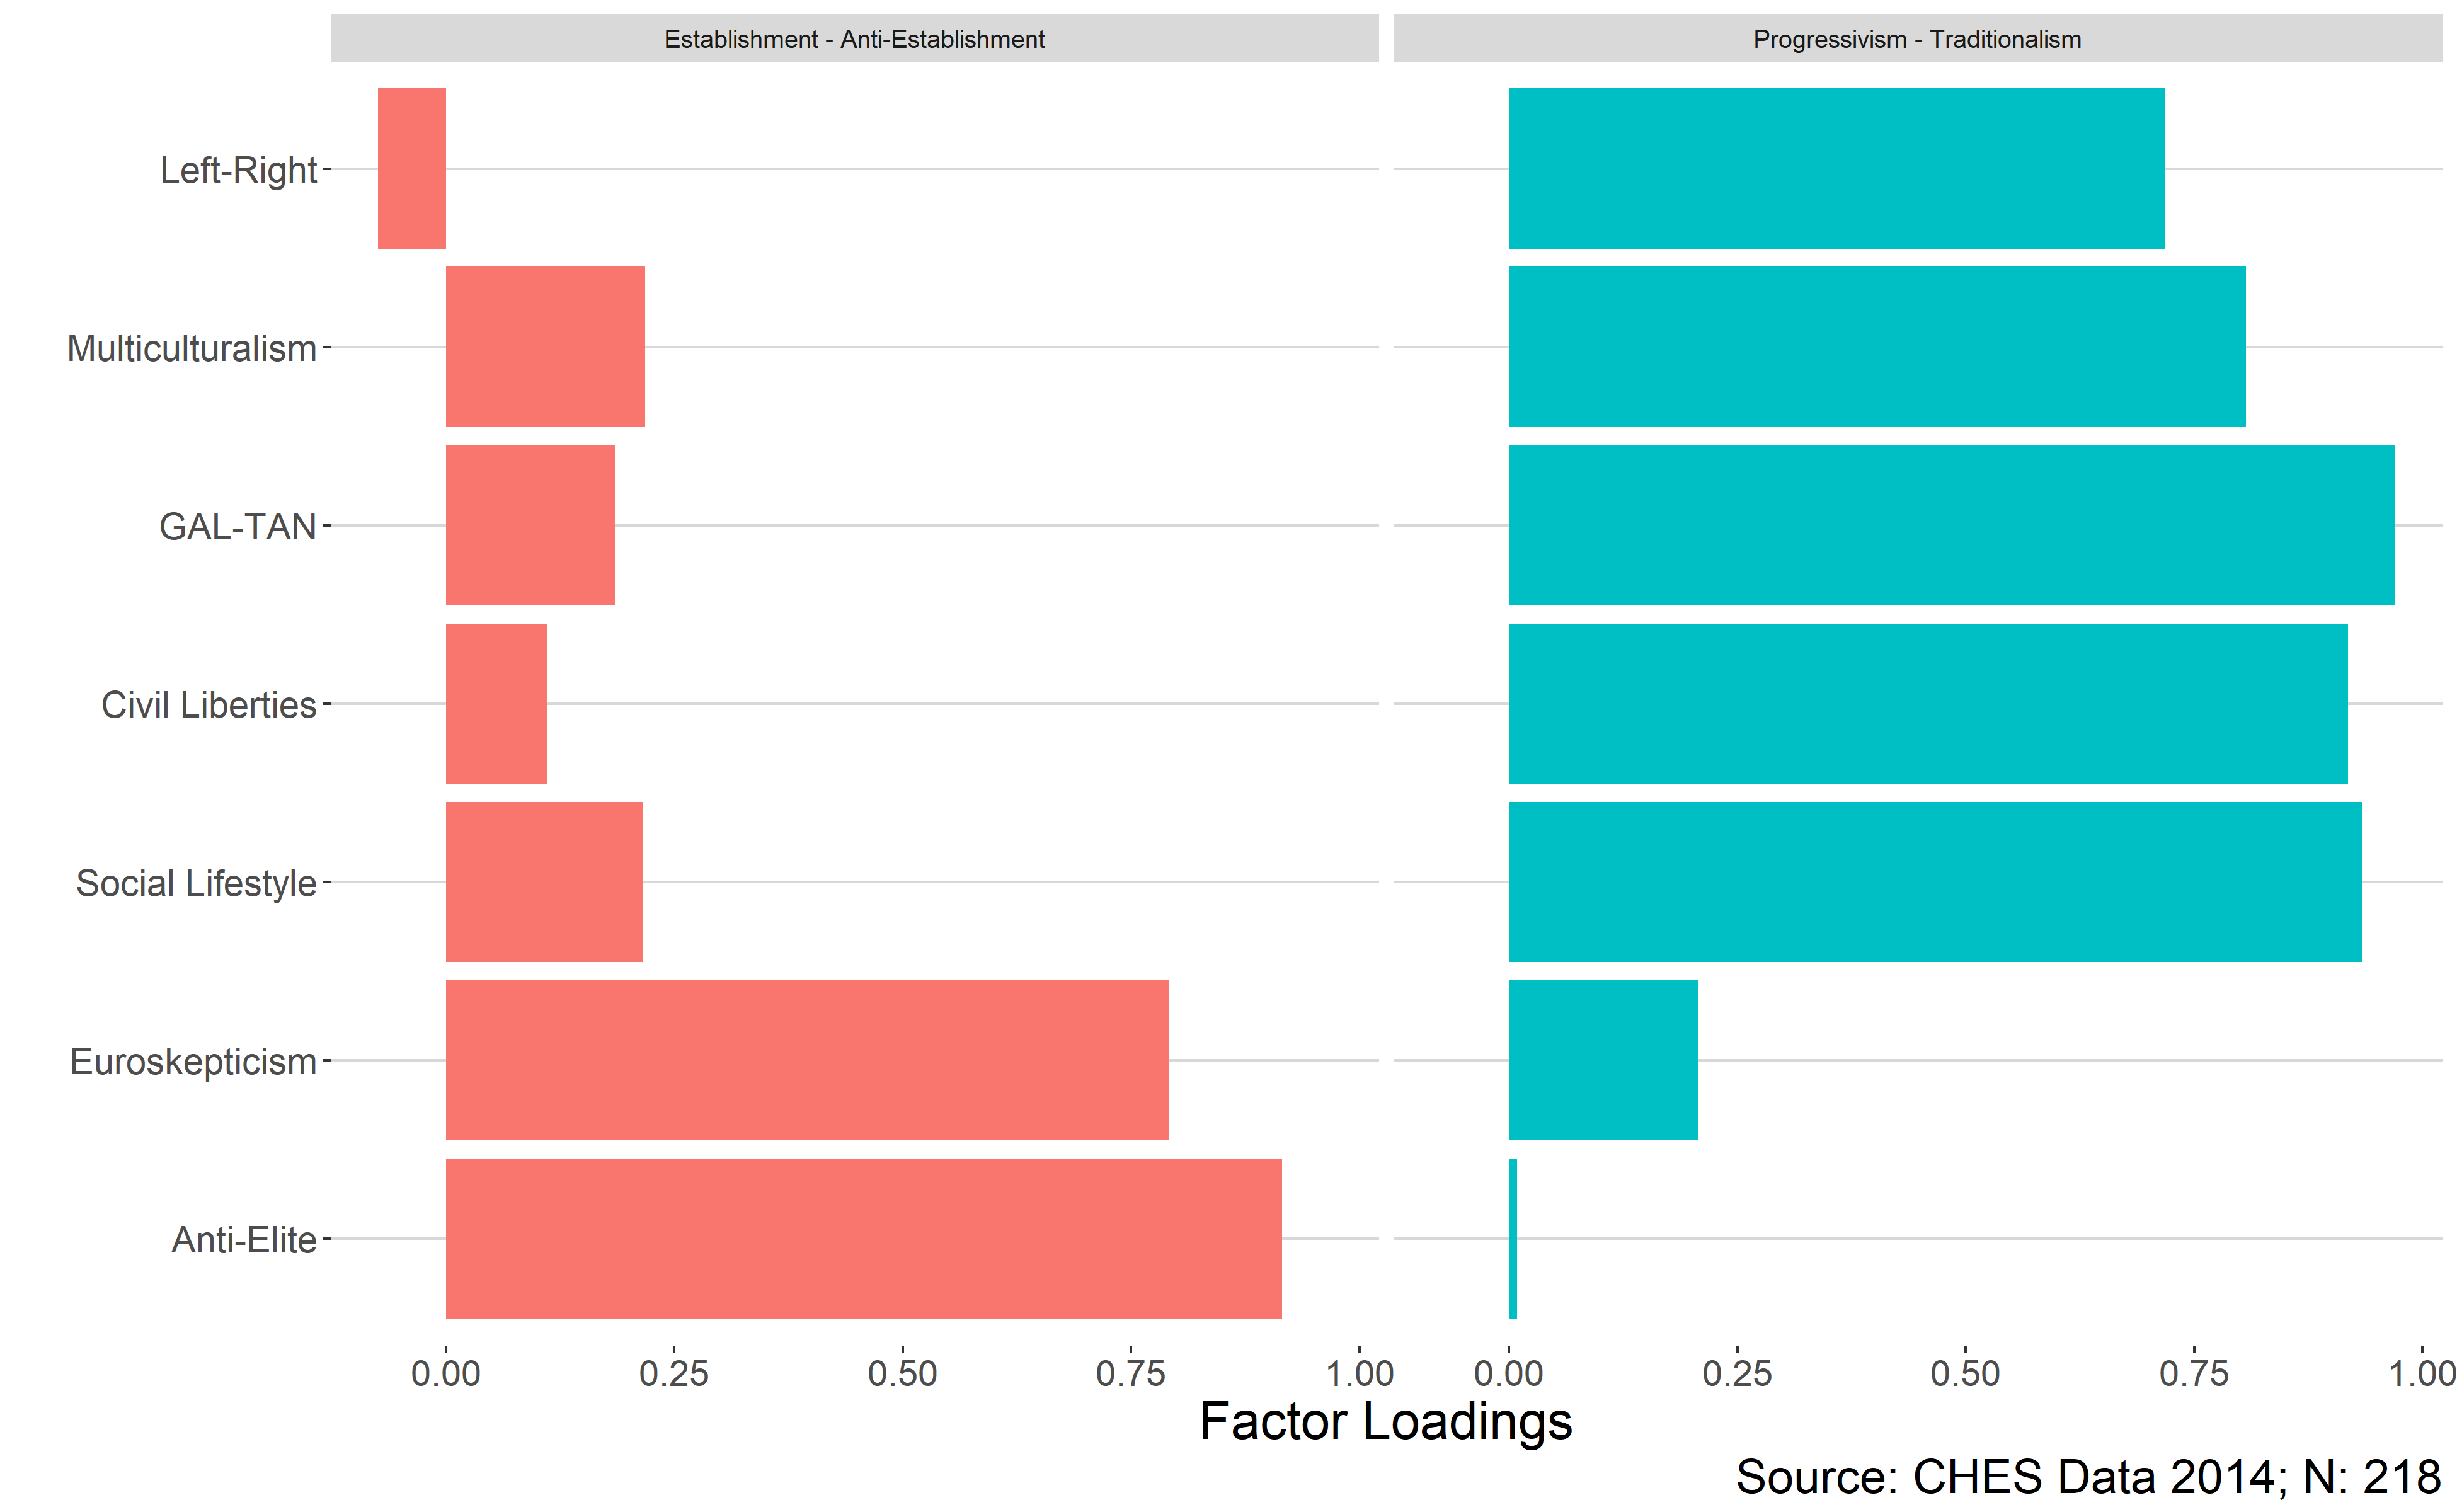
\includegraphics[width=0.8\textwidth]{images/fac_pop}
    \label{fig:mesh1}
\end{figure}

Based on the Kaiser-Criterion, two distinct dimensions are extracted
explaining a total variance of \(0.78\%\). The extracted scales are then
summed into two scales \emph{Establishment vs.~Anti-Establishment} and
\emph{Progressive vs.~Traditionalism}, each standardized from 0 to 100
points to facilitate easy interpretation.

As a next step, we want to extract our traditionalist and progressive
populist parties. This will be done with the help of \emph{k-means
clustering}. K-Means clustering is a very popular form of unsupervised
machine learning that helps with classification problems. The algorithm
producess a \(k\) number of clusters (classification groups), where k is
specified by the researcher. K-Means clustering estimates a centroid
(i.e.~a center) for each group that has the highest \emph{intra-class
similarity} within a given cluster (i.e.~smallest distance from the
centroid) and the lowest \emph{inter-class similarity} with other
specified cluster (i.e.~maximized distance from other cluster
centroids). The resulting clusters have minimal \emph{within cluster
variation} and a maximum of \emph{between cluster variation}.

The classical algorithm for k-means clustering is the Hartigan-Wong
algorithm {[}-@hartigan1979algorithm{]}, where the the total
within-cluster variation is defined as the sum of squared (Euclidean)
distances between data points and the corresponding centroid:

\[W(C_k) = \sum_{x_i \in C_k}(x_i - \mu_k)^2\]

Where \(x_i\) is a data point belonging to the cluster \(C_k\) and
\(\mu_k\) is the mean of values that are classified as cluster \(C_k\)
(centroid).

Each data point \(x_i\) is classified as a specific cluster so that the
sum of squares euclidian distance of the observation to their assigned
cluster centroid \(\mu_k\) is minimized.

\[Within-SS = \sum^k_{k=1}W(C_k) = \sum^k_{k=1}\sum_{x_i \in C_k}(x_i - \mu_k)^2\]

Finally, the total within-cluster sum of square (Within-SS) measures the
appropriateness of the clustering based on how much it can be be
minimized.

Now the algorithm can come into use. As a first step, the algorithm
randomly selects k points from the given data that will be used as
centroids. Next, two steps will be repated iteratively until convergence
is achieved:

\emph{1. Cluster Assignment Step}

\begin{quote}
Using Euclidean distance, the distances to the centroid are calculated
and the data points are classified to be part of a cluster.
\end{quote}

\emph{2. Centroid Update Step}

\begin{quote}
In this step, a new centroid is calculated based on the estimated
clusters. These centroids serve as new starting point and all data
points are reassigned.
\end{quote}

The algorithm converges when the clusters do not change in the next
iteration (the last two iteration produce the same clusters with the
same data points within them).

Finally, the two scales \emph{Establishment vs.~Anti-Establishment} and
\emph{Progressive vs.~Traditionalism} are handed over to the K-means
clustering algorithm. Based on the Gap Statistic method {[}cf.
@tibshirani2001estimating{]}, four clusters are suggested as the optimal
number of clusters.\footnote{Elbow and average silhouette method also
  suggest four clusters as optimal.} Figure \label{fig:gap} shows the
results of the gap statistic that clearly indicate four clusters.

\begin{figure}[!h]
    \centering
    \caption{Results of Gap Statistic Method}
    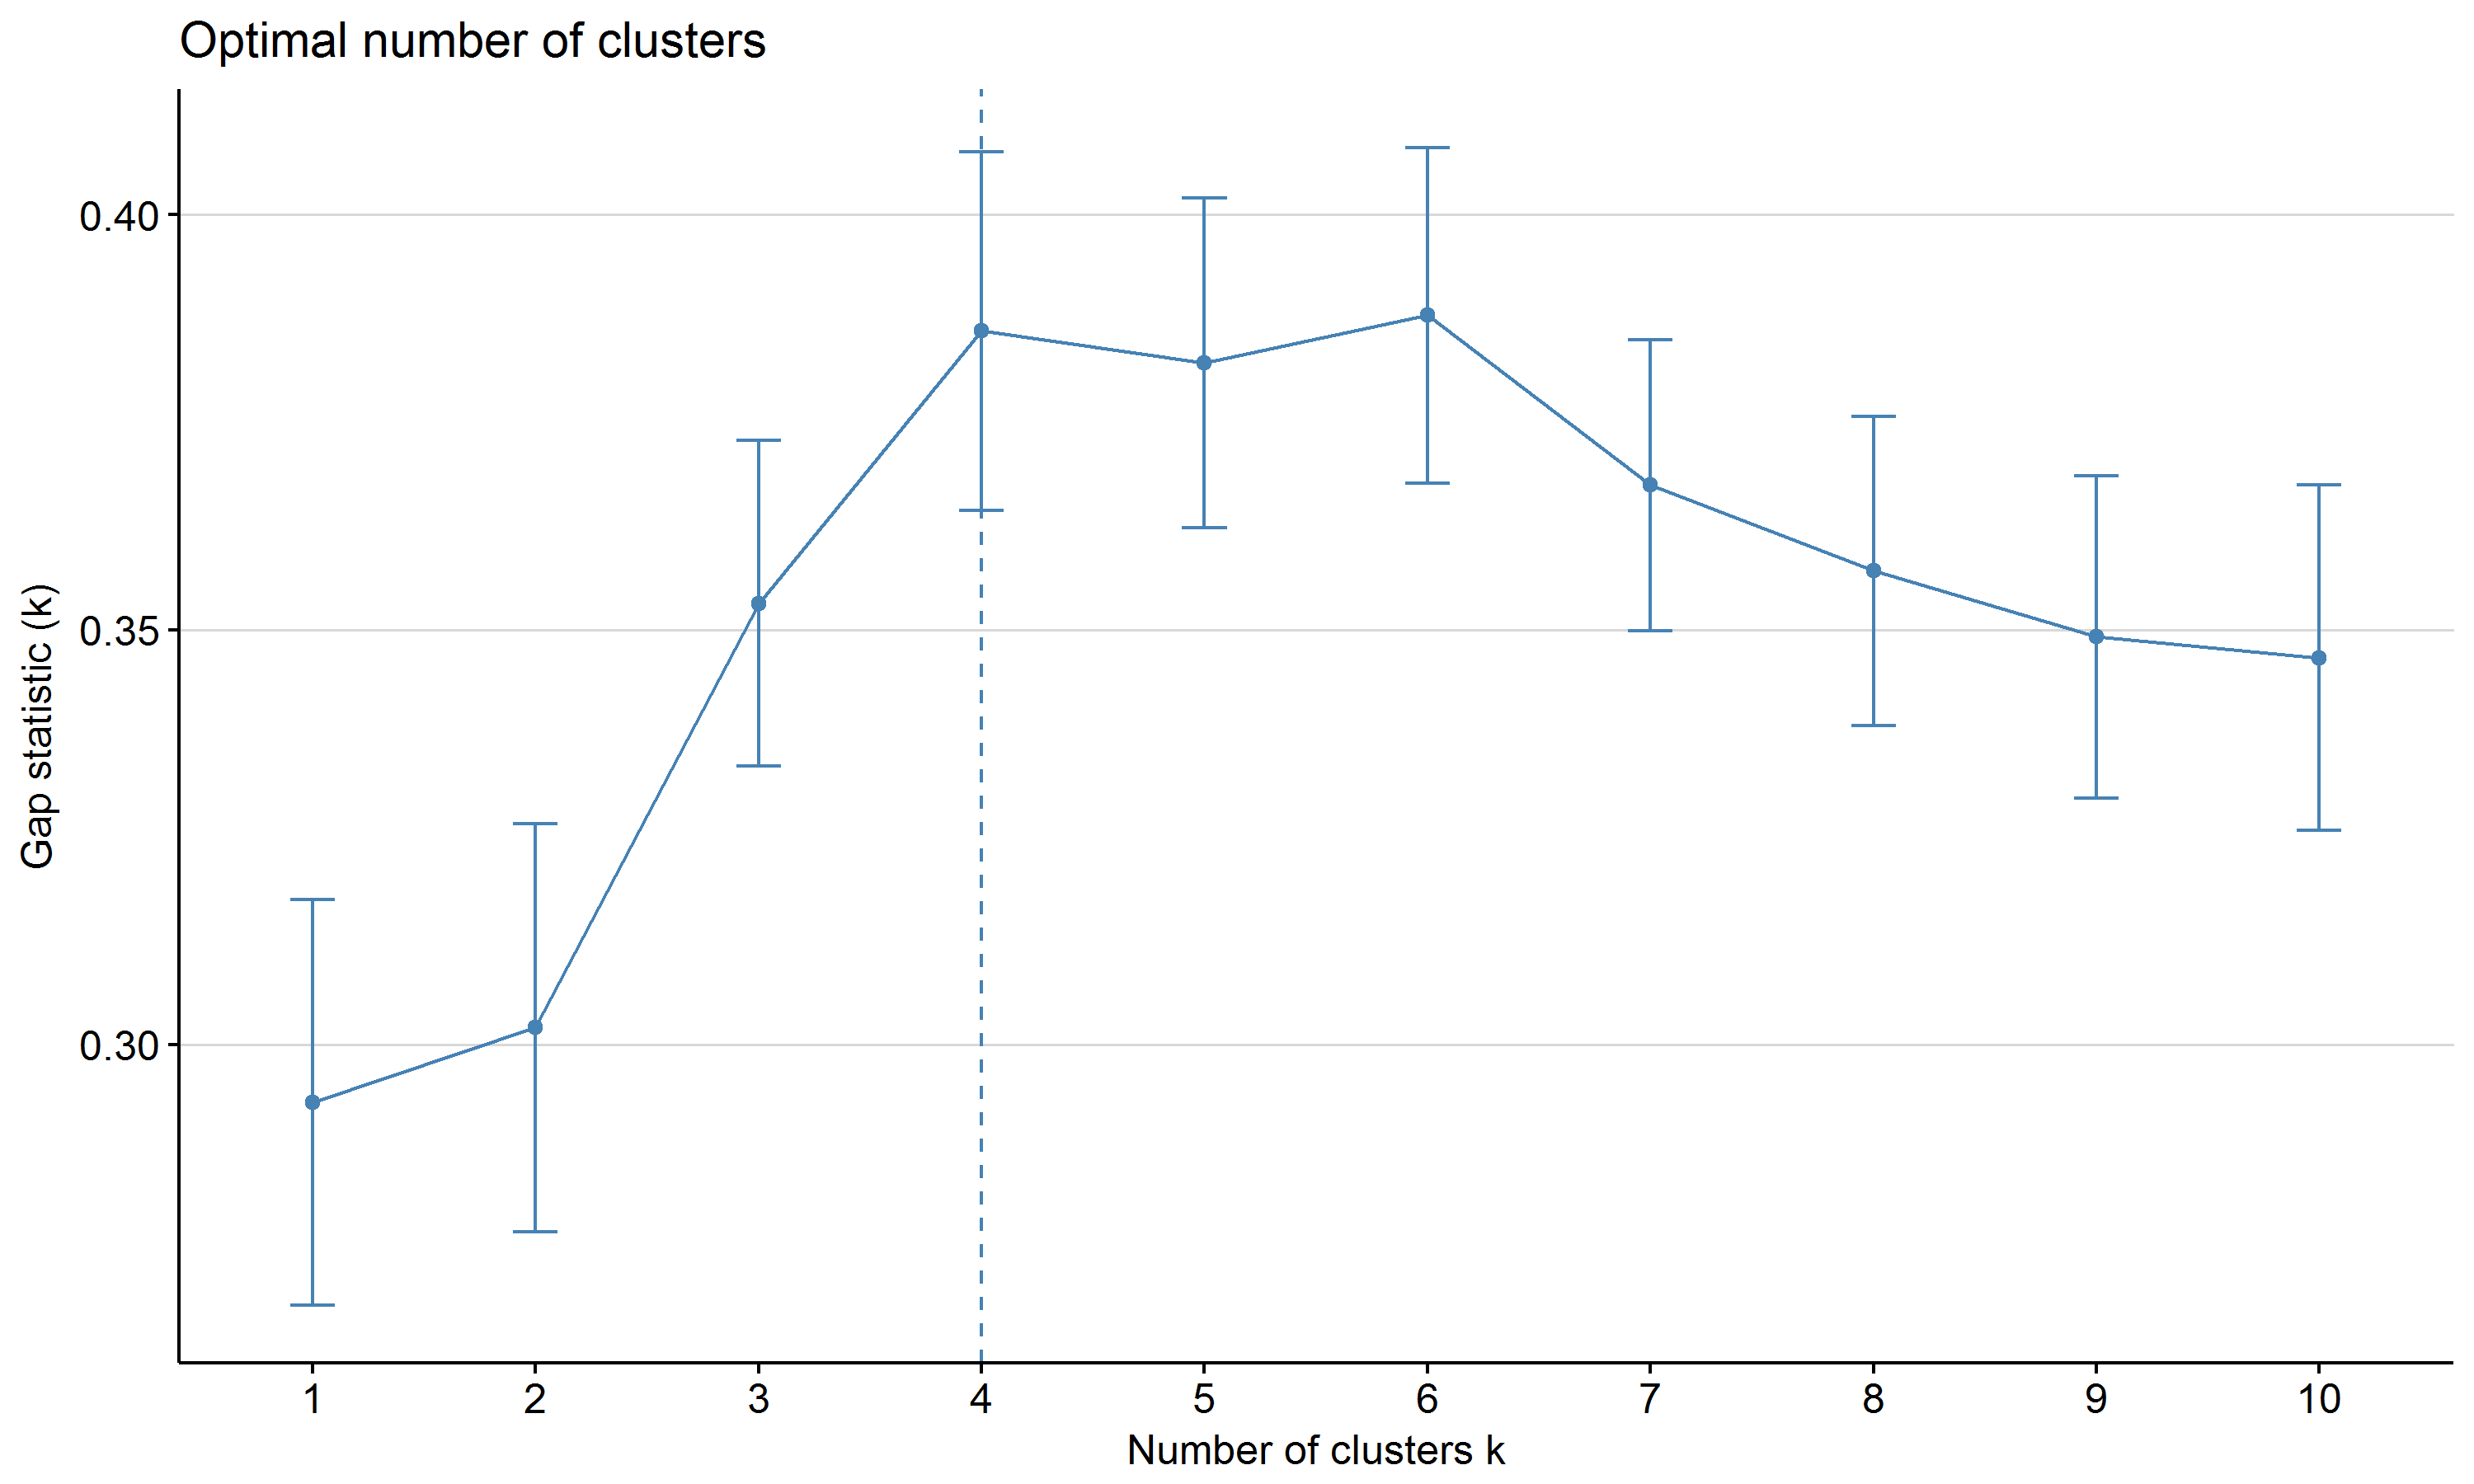
\includegraphics[width=0.8\textwidth]{images/optim_cluster}
    \label{fig:gap}
\end{figure}

The four clusters that are estimated with the help of the k-means
algorithm can be named as traditionalist and progressive populist
parties as well as their two establishment counterparts (establishment
progressives and traditionalists). Together with the clustering method,
the two dimensions can be used to visualize the ideological position of
each Euopean party and its classification, which is illustrated in
Figure \label{fig:alignment}.

\begin{figure}[!h]
    \centering
    \caption{Party Alignment of European Parties}
    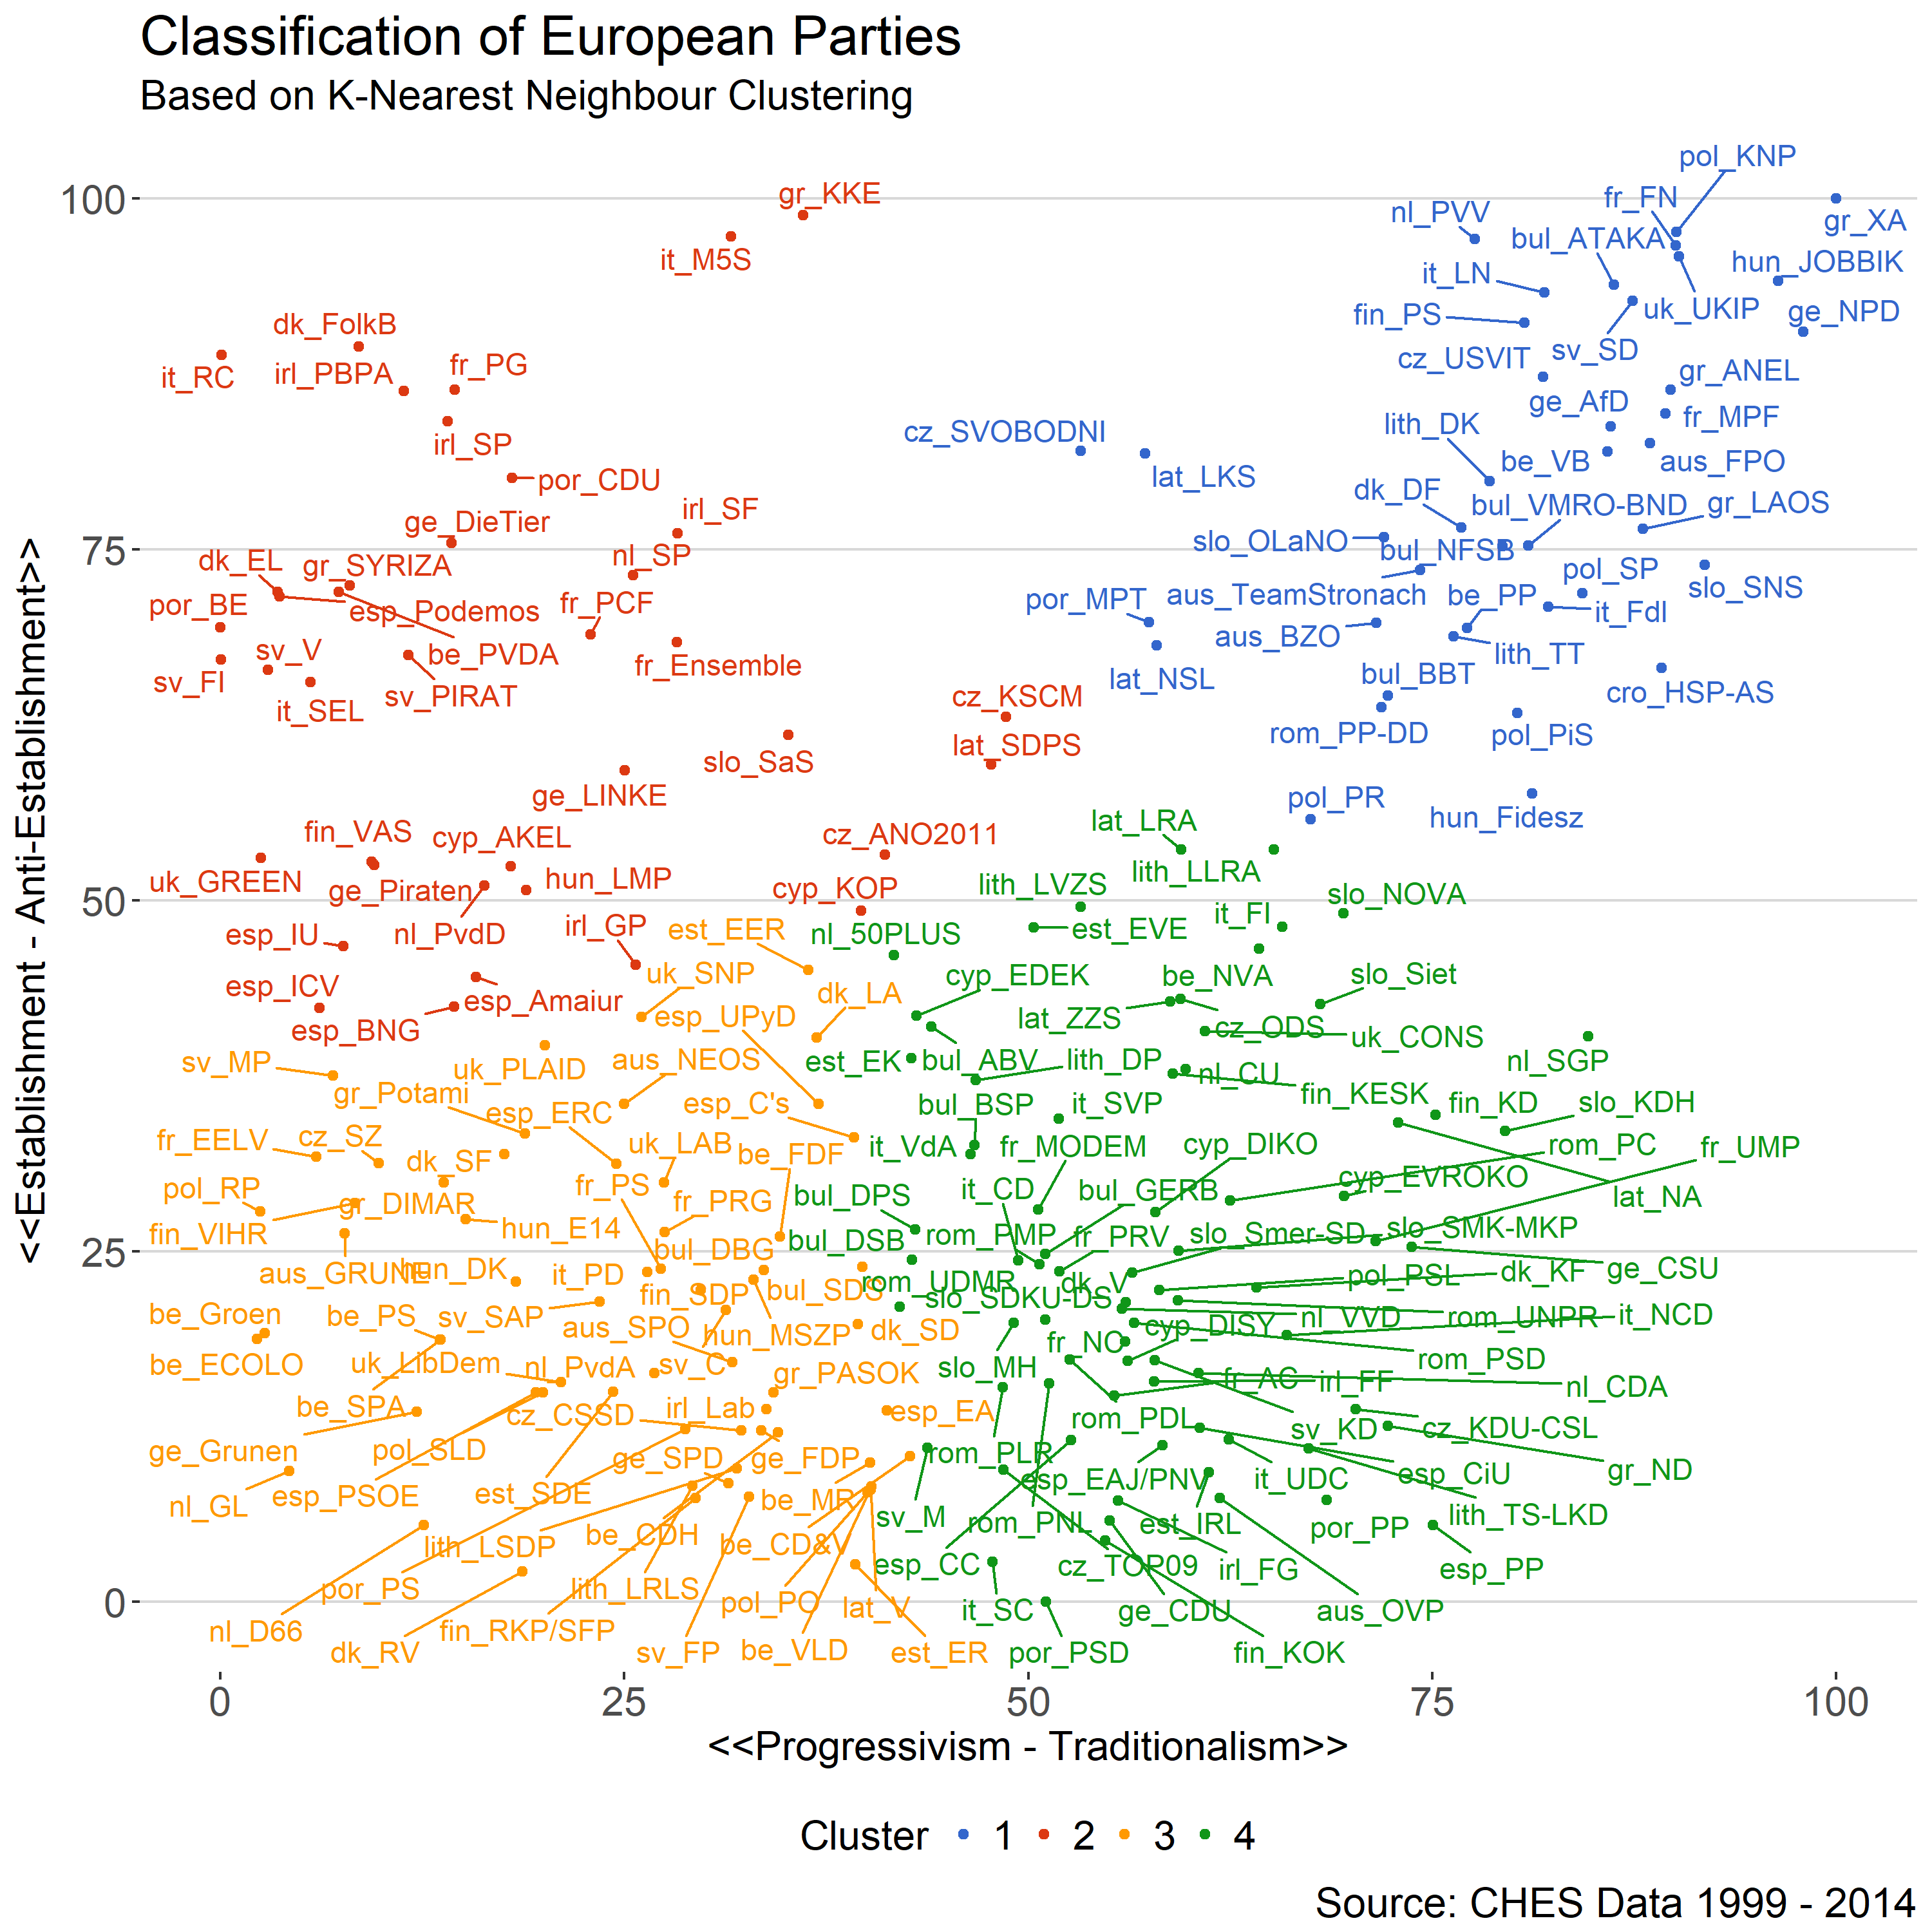
\includegraphics[width=0.8\textwidth]{images/party_alignment_abstract}
    \label{fig:alignment}
\end{figure}

In order to validate the clusters, let's take a look at them in greater
detail and see whether the classified parties fit our theoretical
expectations.

\textbf{TODO:}

\textbf{Top Left} shows progressive populists such as:

\textbf{Syriza}

After winning the parliamentary elections in January 2015, SYRIZA
(\emph{Coalition of the Radical Left}) attempted to carry out the
difficult balancing act between extreme left-wing positions, opposition
to EU imposed austerity and yet supposedly pro-European commitments. In
social policy, Syriza is particularly committed to the socially
disadvantaged in society with policies such as guaranteeing that
unemployed, homeless and low-income people should be allowed to use the
health facilities free of charge or that family reunification should be
made easier for individuals with a migration background.

\textbf{Podemos}

In the general elections held on December 20, 2015, the left-wing
political party Podemos that emerged from a protest movement obtained
20.68\% of the votes and 69 deputies in the whole of the State. The
Spanish ``Indignados'', the ``indignants'' of the Podemos movement,
practice critique of globalization and capitalism often symbolized in
the overarching EU bureacracy. Among other measures, they defend
abortion, want to stop house evictions, suppress church privileges,
promote renewable energies and are in favor of curbing nuclear energy.
With regard to political parties, they propose to stop gauging, reduce
subsidies and expand restrictions on connections between politicians and
companies.

\textbf{Red--Green Alliance (Denmark)}

The Red--Green Alliance (Enhedslisten) was formed as a collaboration
between the Left Socialists (VS), the Danish Communist Party (DKP) and
the Socialist Labor Party (SAP) in 1989. During the last parliamentary
elections in 2015, the Red--Green Alliance gained 7,8\% of the popular
vote. Enhedslisten does not stand in European elections, but supports
Folkebevægelsen mod EU (\emph{Popular Movement against the EU}), a
heavily anti-EU political party that only competes for the European
elections. The party attaches great importance to combating social
inequality and poverty, as well as advocating strengthening and
expanding the welfare state. Politically, the party is in favor of more
space for all forms of diversity, including gender, sexuality,
disability and ethnic background.

\textbf{DESCRIBE THEM}

\textbf{Top Right} shows traditionalist populists such as:

\textbf{AfD}

The alternative for Germany (AfD) is a political party founded in 2013
in Germany. As of 2014, it gradually moved into 14 state parliaments and
in the 2017 general election, the AfD received 12.6\% of the vote and
thus became the third strongest force and the strongest opposition party
in the German Bundestag. Regarding the EU, they have been in favor of
renationalization of policies that are currently situated in the EU. The
AfD represents conservative-antifeminist positions in gender politics
and rejects gender equality policies and relies thereby on Christian
fundamentalist and nationalist ideas. According to the AfD, Islam does
not belong to Germany. In particular, the party calls for a ban on
minarets and the face veiling.

\textbf{Front National}

\textbf{UKIP}

\textbf{DESCRIBE THEM}

\textbf{Bottom left and bottom right} shows progressive and
traditionalist establishment parties:

German SPD and CDU, Labour Party and Conservatives UK, SOME FRENCHIES

\textbf{DESCRIBE THEM}

Given that the distinction between kinds of establishment parties is not
of greater interest to us, we will merge progressive and traditionalsit
establishment parties into a single establishment party group.

Our measure of populism correlates well with different similar
classification methods.

(TODO:) CORRELATION WITH OTHER MEASURES

(TODO:) ONLY INCLUDE PARTIES THAT ARE USED LATER ON

A full list of used parties as well as their respective affiliations can
be found in the appendix.

(TODO: TABLE that shows the individuals scores)

\subsubsection{Dependent Variable: Support for Populist
Parties}\label{dependent-variable-support-for-populist-parties}

\textbf{TODO:}

(TODO:) INCLUDE ALL ESS ROUNDS

The European Social Survey data is such and such.

\begin{itemize}
\tightlist
\item
  from when to when
\item
  which countries
\item
  how many parties
\item
  actual operationaliztion
\end{itemize}

After the successful classification, we combine the clusters from the
CHES data with the \emph{European Social Survey} (ESS) Round 5 -- 8. We
decided to use only these dates, as we expect the years after the
European financial crisis (2008-09) to be more homoegenous in terms of
populism. Two variables will be used to measure our dependent variable
\emph{Support for Populist Parties}:

\emph{1. What party did you vote for in the last national election?}

\emph{2. Which party is closest to your views?}

A respondent that either voted for or indicated that they feel closest
to a specific party, will be classified as either supporting a
progressive or traditionalist populist or an establishment party, based
on the clusters generated by the K-means alghorithm. If it is the case
that a person voted for a party but felt close to a different party, we
decided to classify said person as a supporter of the party that it felt
most close to (thus ranking their vote as less indicative of their
support). This is based on the assumption that many voters have an
incentive to vote strategically and they might end up voting for an
establishment party even though they actually support a populist party
(TODO: \textbf{CITATION}).

After the merging is completed we are left with XXX respondents from 24
European countries.

TODO: \textbf{Descriptives?}

\subsubsection{Independent Variables: Cultural and Economic
Explanations}\label{independent-variables-cultural-and-economic-explanations}

TODO: \textbf{Description of INDEPENDENT VARIABLES?}

Next, the hypotheses will be operationalized with corresponding ESS
variables. \emph{Economic deprivation} will be captured with two
variables: Economic Insecurity and Unemployment (0/1). The
\emph{cultural value hypothesis} will be measured with an index for
anti-immigration sentiment and four Schwartz Human Value dimensions
(Openness to Experience, Conservation, Self-Enhancement and
Self-Transendence). The models further include common socio-demographic
control variables, for example, age, education and sex but also includes
a Left-Right Scale, Religiosity, Government Satisfaction, Minority
Status, Trust in the EU \& UN and Rural vs.~Urban. Lastly, regional
dummies (East, West, North and South Europe) and time dummies for each
year will be included in the model as controls.

A more detailed description of the used variables as well as general
statistics of all the used variables can be found in the Appendix.

\textbf{TODO: How many point scales?}

\textbf{CHECK THIS} All models were checked by tolerance tests to be
free of problems of multicollinearity..

\subsection{Statistical Methodology}\label{statistical-methodology}

Here comes a description of the multinomial model (might need to change
the name of the title)

Multinomial logistic regression is an extension of binary logistic
regression, which makes it possible to predict three or more outcomes of
a variable. In this case, each category of the variable of interest will
be compared to the \emph{reference category} that is specified by the
researcher with the consequence that estimated parameters (logits and/or
odds ratios) are interpreted in reference to that category.

In the multinomial logit model we assume that the log-odds of each
response follow a linear model

\[\eta_{ij} = \log\frac{\pi_{ij}}{\pi_{iJ}} = \alpha_j + \boldsymbol{x}_i'\boldsymbol{\beta}_j\]

where \(\alpha_j\) is a constant and \(\beta_j\) is a vector of
regression coefficients, for \(j = 1, 2, \ldots, J-1\). Note that we
have written the constant explicitly, so we will assume henceforth that
the model matrix \(\boldsymbol{X}\) does not include a column of ones.

This model is analogous to a logistic regression model, except that the
probability distribution of the response is multinomial instead of
binomial and we have \(J-1\) equations instead of one. The \(J-1\)
multinomial logit equations contrast each of categories
\(j = 1, 2, \ldots, J-1\) with category \(J\), whereas the single
logistic regression equation is a contrast between successes and
failures. If \(J=2\) the multinomial logit model reduces to the usual
logistic regression model.

Note that we need only \(J-1\) equations to describe a variable with
\(J\) response categories and that it really makes no difference which
category we pick as the reference cell, because we can always convert
from one formulation to another.

Theoretically a multilevel model would have been needed to estimate the
model properly, but given that there are some countries with almost none
or no populist supporters in our data, this would lead to problems. In
order to still account for the hierarchical order of our data, we
decided to use regional variables of Europe, based on the four
classifications by the UN: Eastern, Western, Southern and Northern
Europe.

\subsection{Descriptives}\label{descriptives}

\begin{landscape}
\vspace*{\fill}
\begin{figure}[htpb]
  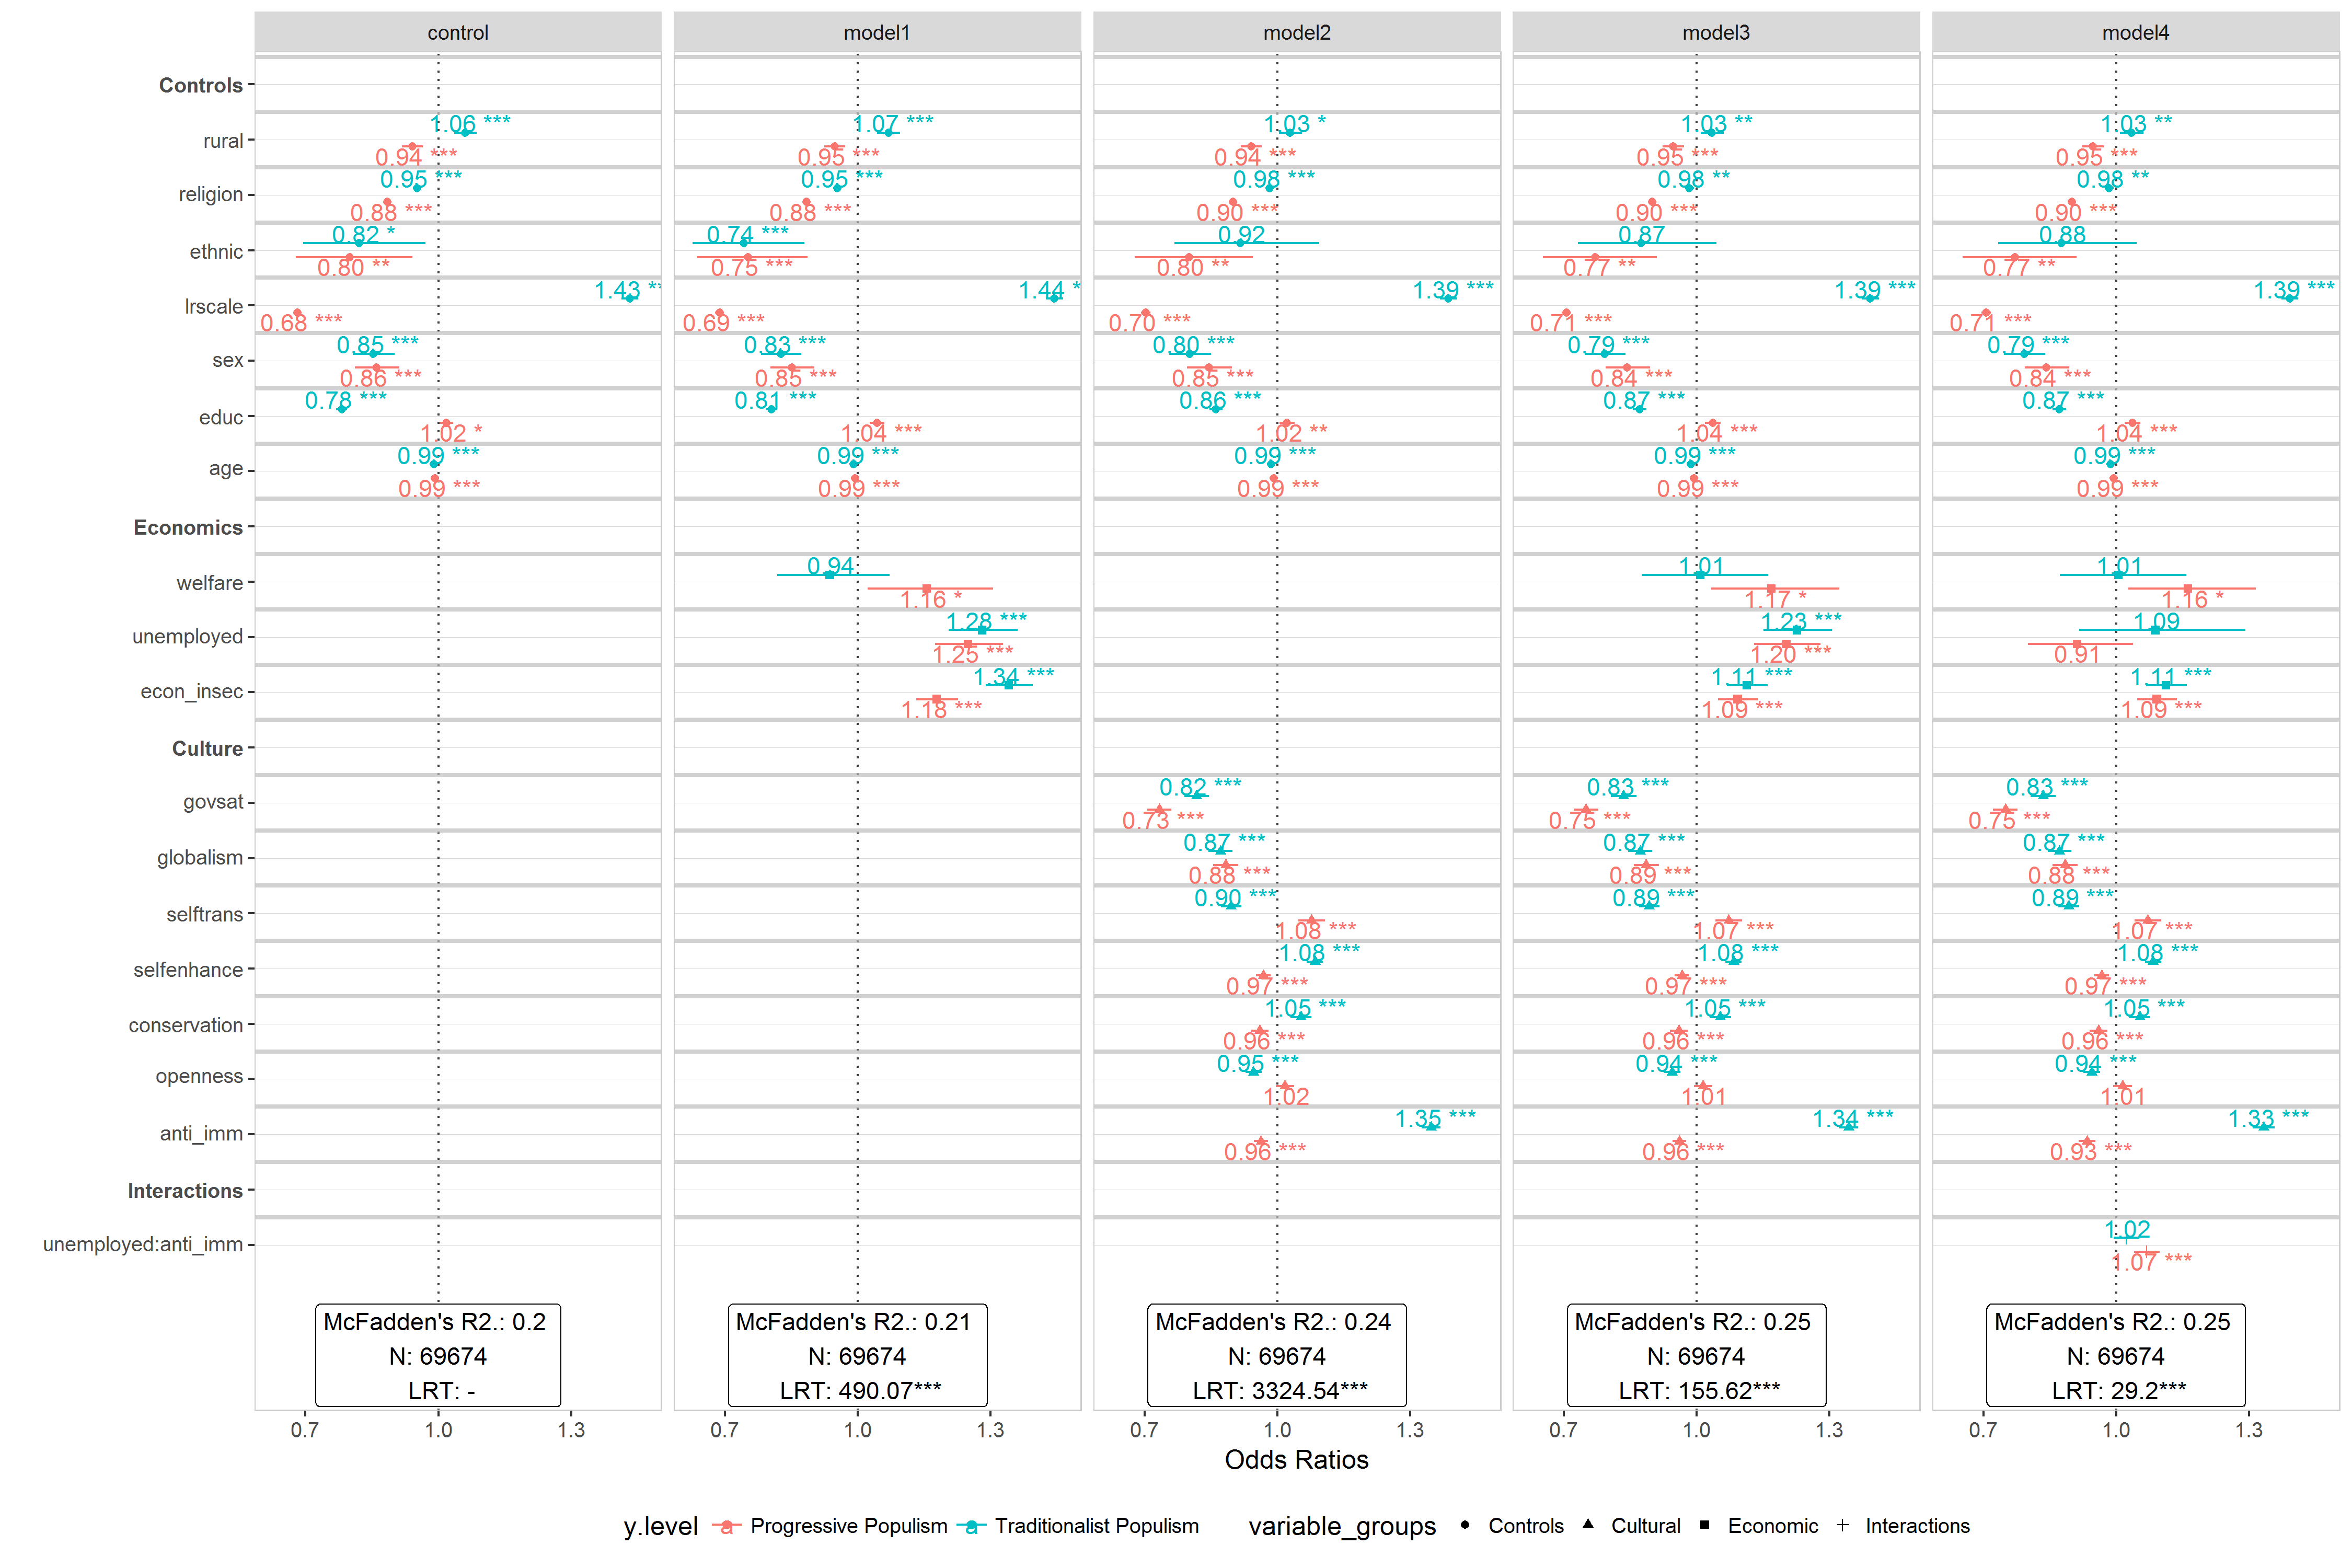
\includegraphics[height=1.2\textheight, width=1.5\textwidth]{images/onebigmotherfucker.png}
  \caption{Functional Decomposed Data Structure}
\end{figure}
\vfill
\end{landscape}

\textbf{TODO:}

\begin{itemize}
\tightlist
\item
  Populist Parties by Region
\item
  Populist Parties by Country (map)
\end{itemize}

Descriptive Statistics and Exploratory Evaluation of the Hypotheses

\subsection{Multinomial Logistic
Regression}\label{multinomial-logistic-regression}

Here comes the Analysis Part

\textbf{TODO}

\begin{itemize}
\tightlist
\item
  Plots: \emph{descriptives} Regional Plot (how many populists per
  region) Boxplot: age + educ + sex + lrscale+ religion + rural Populist
  Parties by Country (map) \emph{analysis} Coefficent Plots (one big
  motherfucker) Probability Plots for the main hypotheses
\end{itemize}


\end{document}
